\documentclass[crop,tikz]{standalone}
\usetikzlibrary{arrows.meta,calc,decorations.markings,math,arrows.meta}

\begin{document}
	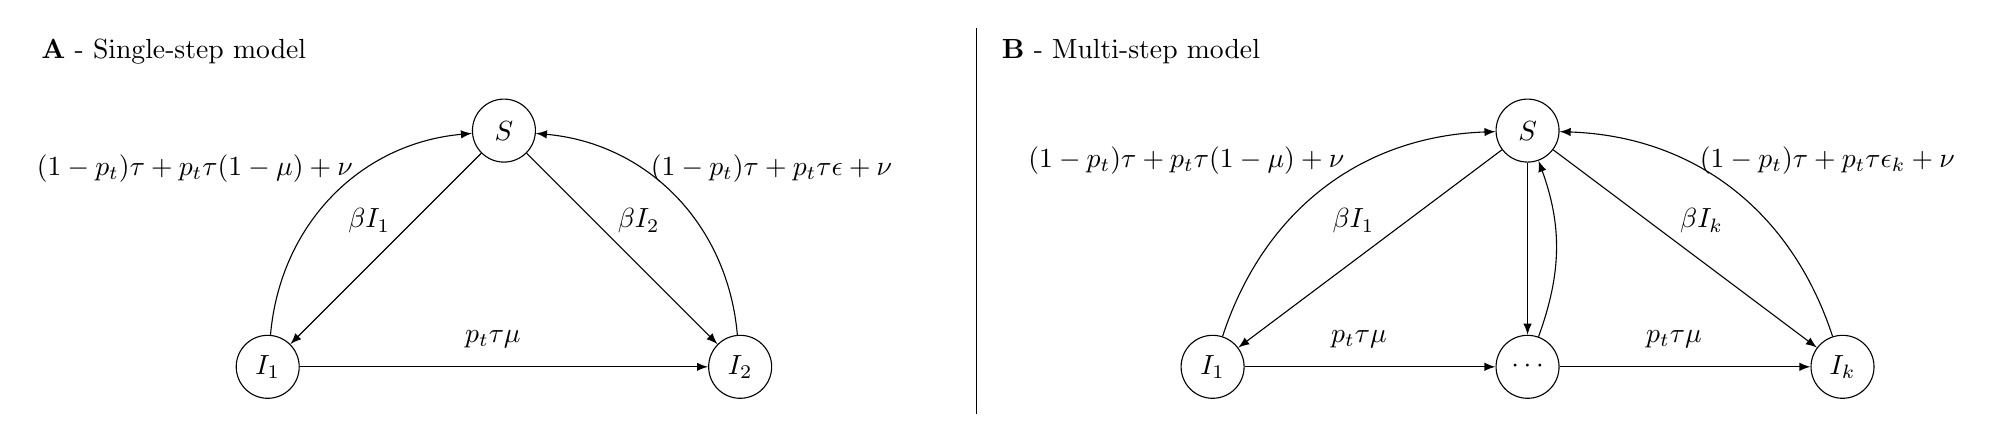
\begin{tikzpicture}

	\node[anchor=west] at (-6,1) {\textbf{A} - Single-step model};
	\node[circle, draw, inner sep=0pt, minimum size=.8cm] (S) at (0,0) {$S$};
	\node[circle, draw, inner sep=0pt, minimum size=.8cm] (Ik1) at (-3,-3) {$I_1$};
	\node[circle, draw, inner sep=0pt, minimum size=.8cm] (Ik2) at (3,-3) {$I_2$};
	
	\draw[->,>=latex] (S) -- node[yshift=10,xshift=-6] {$\beta I_1$} (Ik1);
	\draw[->,>=latex] (S) -- node[yshift=10,xshift=6] {$\beta I_2$} (Ik2);
	\draw[->,>=latex] (Ik1) -- node[yshift=10,xshift=-4] {$p_t\tau \mu$} (Ik2);
	\draw[->,>=latex] (Ik1) edge[bend left=40] node[yshift=10,xshift=-50] {$(1-p_t) \tau + p_t \tau (1-\mu)  +\nu$} (S);
	\draw[->,>=latex] (Ik2) edge[bend left=-40] node[yshift=10,xshift=35] {$(1-p_t) \tau + p_t \tau \epsilon + \nu$} (S);	
	
	\node[anchor=west] at (6.2,1) {\textbf{B} - Multi-step model};
	\node[circle, draw, inner sep=0pt, minimum size=.8cm] (bS) at (13,0) {$S$};
	\node[circle, draw, inner sep=0pt, minimum size=.8cm] (bIk1) at (9,-3) {$I_1$};
	\node[circle, draw, inner sep=0pt, minimum size=.8cm] (bIk2) at (13,-3) {$\cdots$};	
	\node[circle, draw, inner sep=0pt, minimum size=.8cm] (bIk3) at (17,-3) {$I_k$};
	
	\draw[->,>=latex] (bS) -- node[yshift=10,xshift=-6] {$\beta I_1$} (bIk1);
	\draw[->,>=latex] (bS) -- (bIk2);
	\draw[->,>=latex] (bS) -- node[yshift=10,xshift=6] {$\beta I_k$} (bIk3);
	\draw[->,>=latex] (bIk1) -- node[yshift=10,xshift=-4] {$p_t\tau \mu$} (bIk2);
	\draw[->,>=latex] (bIk2) -- node[yshift=10,xshift=-4] {$p_t\tau \mu$} (bIk3);
	\draw[->,>=latex] (bIk1) edge[bend left=35] node[yshift=10,xshift=-50] {$(1-p_t) \tau + p_t \tau (1-\mu)  +\nu$} (bS);
	\draw[->,>=latex] (bIk3) edge[bend left=-35] node[yshift=10,xshift=35] {$(1-p_t) \tau + p_t \tau \epsilon_k + \nu$} (bS);
	\draw[->,>=latex] (bIk2) edge[bend left=-20] (bS);	
	
	\draw (6,1.3) -- (6,-3.6);
	
\end{tikzpicture}
\end{document}